% !TEX program = xelatex
% vim:foldmethod=marker:foldmarker=<<<,>>>
\documentclass[compress,aspectratio=169]{beamer}

%<<< Preamble
\usepackage[english]{babel}
\usepackage{metalogo}
\usepackage{listings}
\usepackage{fontspec}
\usepackage{amsmath, amssymb, bm}
\usepackage{stackrel}
\usepackage{tikz}
\usepackage{unicode-math}
\usepackage{subcaption}


\usepackage[theme=nord,charsperline=60,linenumbers]{jlcode}
\usetheme{Nord}

% Uncomment lines bellow for light theme
% \usepackage[charsperline=60,linenumbers]{jlcode}
% \usetheme{Boadilla}

\setmainfont{Roboto}
% \setsansfont{DejaVu Serif}
% \setmonofont{CaskaydiaCove Nerd Font Mono}
\setmonofont{JuliaMono}

\setbeamercolor{mybullet}{use=itemize item.fg,bg=itemize item.fg,fg=itemize item.fg}

\makeatletter
\def\verbatim@nolig@list{}
\newcommand\pin{%
\parbox[t]{10pt}{\raisebox{0.2pt}{\usebeamercolor[fg]{mybullet}{$\ast$}}}}
\makeatother

\newcommand{\E}[1]{\ensuremath{E\left\{#1\right\}}}
\newcommand{\norm}[1]{\ensuremath{\lVert#1\rVert}}
\newcommand*{\thead}[1]{\multicolumn{1}{c}{\fseries #1}}

\newfontfamily\tabulartext[SizeFeatures={Size=6}]{Roboto}

\hypersetup{
    colorlinks=true,
    urlcolor=NordBlue
}

\DeclareMathOperator*{\argmax}{argmax}
\DeclareMathOperator*{\Var}{Var}
\DeclareMathOperator*{\test}{\gtrless}

\AtBeginDocument{
    \fontsize{8}{12}
    \selectfont

}

\AtBeginSection[]
{
    \begin{frame}[c,noframenumbering,plain]
        \tableofcontents[sectionstyle=show/hide,subsectionstyle=show/show/hide]
    \end{frame}
}


\AtBeginSubsection[]
{
    \begin{frame}[c,noframenumbering,plain]
        \tableofcontents[sectionstyle=show/hide,subsectionstyle=show/shaded/hide]
    \end{frame}
}
%>>>

\title{Project III}
\subtitle{MIMO Pulse-echo imageing}
\author{Simon Andreas Bjørn}
\date{May 4, 2023}

\begin{document}

\begin{frame}[plain,noframenumbering]
    \maketitle
\end{frame}

\begin{frame}[fragile] % <<< 1 - Pulse compression
    \frametitle{1 - Pulse compression}
    We want to implement pulse compression (match filtering).
    
    The implementation of pulse compression looks like this
    \begin{jllisting}[gobble=8]
        # Match filter      |--Perform Match Filter--||-----Get the positive lag------|
        match_filter(x, y) = conv(x, reverse(conj(y)))[length(y)÷2+1:end-(length(y)÷2)]
    \end{jllisting}
    We can find the theoretical time-resolution in seconds for the sequence after
    pulse compression by using the bandwidth $B$ which is given by
    $$
        \delta\tau = \frac{1}{B}
    $$
    \begin{jllisting}[gobble=8]
        δτ = 1/B |> toUnit(u"ms")
        @show δτ; # -> δτ = 0.1 ms
    \end{jllisting}
    So the theoretical time-resolution in seconds are $0.0001s$ or $0.1ms$
\end{frame}
% >>>

\begin{frame}[fragile] % <<< 1 - Test Pulse compression
    \frametitle{1 - Test Pulse compression}
    We want to test the pulse compression on a channel from the \jlinl{tdma_data}
    and plot before and after filtering.

    First, we create the transmitted LFM pulses as defined in the
    assignment.
    \begin{jllisting}[gobble=8]
        α = B/Tₚ
        S_up   = (t -> @. exp(1im*2π*((fc - B/2)*t + α*t^2/2)))(0s:1/fs:Tₚ);
        S_down = (t -> @. exp(1im*2π*((fc + B/2)*t - α*t^2/2)))(0s:1/fs:Tₚ);
    \end{jllisting}
    \begin{columns}
        \begin{column}{0.5\textwidth}
            Then, we apply \jlinl{match_filter()} on the data
            \begin{jllisting}[gobble=16]
                raw_signal = tdma_data[:,1,1]
                match_signal = match_filter(raw_signal, S_up)
            \end{jllisting}
        \end{column}
        \begin{column}{0.5\textwidth}
            \begin{figure}
                \includegraphics[width=\columnwidth]{"../1.pdf"}
            \end{figure}
        \end{column}
    \end{columns}
\end{frame}
% >>>

\begin{frame}[fragile] % <<< 1 - Pulse compression measured performance
    \frametitle{1 - Pulse compression measured performance}
    Measure the FWHM of the pulse compression around the peak to find performance.
    \begin{jllisting}[gobble=8]
        # Assumes only 1 peak at interval x
        fwhm(x) = (count(a -> a >= 0.5maximum(x), x)+2) / fs
    \end{jllisting}

    \begin{columns}
        \begin{column}{0.5\textwidth}
            Evaluating \jlinl{fwhm(x)} on \jlinl{match_signal} we find the
            measured time-resolution
            \begin{jllisting}[gobble=16]
                P_match = @. abs(match_signal)^2
                τₚ = fwhm(P_match) |> toUnit(u"ms")
                @show τₚ; # -> τₚ = 0.1 ms
            \end{jllisting}
            We see that this matches exactly with the theoretical resolution.
        \end{column}
        \begin{column}{0.5\textwidth}
            \begin{figure}
                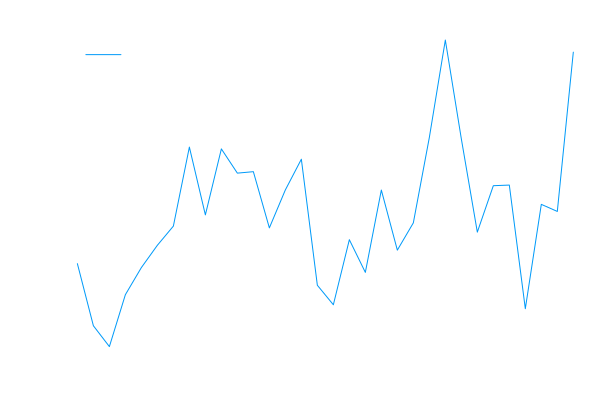
\includegraphics[width=\columnwidth]{"../2.pdf"}
            \end{figure}
        \end{column}
    \end{columns}
\end{frame}
% >>>

\begin{frame}[fragile] % <<< 2 - Virtual Arrays
    \frametitle{2 - Virtual Arrays}
    We want to construct a virtual array of our setup.
    We know that each virtual sensor is defined as
    $$
        V_x = \frac{(R_x+T_x)}{2}
    $$
    Mapping the receiver positions on each transmit, we get 2 groups of virtual
    sensors.
    \begin{jllisting}[gobble=8]
        v_pos1 = map(x->(x+tₓ_pos[1]) / 2, rₓ_pos)
        v_pos2 = map(x->(x+tₓ_pos[2]) / 2, rₓ_pos)
        v_pos = sort([v_pos1; v_pos2])
    \end{jllisting}
    Plotting these virtual arrays we get the following plot
    \begin{figure}
        \includegraphics[width=\columnwidth]{"../3.pdf"}
    \end{figure}
\end{frame}
% >>>

\begin{frame}[fragile] % <<< 2 - Theoretical resolution
    \frametitle{2 - Theoretical resolution estimation}
    We now want to estimate the theoretical resolution in both axial and lateral
    direction.
    \begin{columns}
        \begin{column}{0.5\textwidth}
            \begin{itemize}
                \item Theoretical lateral resolution in radians
                    \begin{jllisting}[gobble=24]
                        λ = c/fc |> toUnit(m)
                        L₁ = v_pos1[end] - v_pos1[1]
                        Lₐ = v_pos[end] - v_pos[1]

                        @show δβ₁ = λ/2L₁; # -> δβ₁ = 0.0323
                        @show δβₐ = λ/2Lₐ; # -> δβₐ = 0.0317
                    \end{jllisting}
                \item Approximate lateral resolutin at 4m distance
                    \begin{jllisting}[gobble=24]
                        @show δβ₁_4m = δβ₁*4m; # -> δβ₁_4m = 0.129 m
                        @show δβₐ_4m = δβₐ*4m; # -> δβₐ_4m = 0.127 m
                    \end{jllisting}
            \end{itemize}
        \end{column}
        \begin{column}{0.5\textwidth}
            \begin{itemize}
                \item Axial pulse-echo resolution
                    \begin{jllisting}[gobble=24]
                        δr = c/2B |> toUnit(m);
                        @show δr; # -> δr = 0.017 m
                    \end{jllisting}
            \end{itemize}
        \end{column}
    \end{columns}
\end{frame}
% >>>

\begin{frame}[fragile] % <<< 3 - Delay-And-Sum
    \frametitle{3 - Delay-And-Sum}
    \begin{columns}
        \begin{column}{0.55\textwidth}
            Implementation of DAS
            \begin{jllisting}[gobble=16]
                function DAS(grid, channel_data, tx, rx)
                    result = zeros(ComplexF64, size(grid))
                    for k in eachindex(tx)     # For each transmit
                        for j in eachindex(rx) # For each receiver
                            # For each pixel
                            for i in CartesianIndices(grid) 
                                # Get Delay
                                rᵣ = norm([rx[j], 0m] .- grid[i])
                                rₜ = norm([tx[k], 0m] .- grid[i])
                                τ = (rₜ+rᵣ)/c
                                # Get index from delay
                                τ_idx = round(Int, τ * fs)
                                # Sum over delayed signal
                                result[i] += channel_data[τ_idx,j,k]
                            end
                        end
                    end
                    result
                end;
            \end{jllisting}
        \end{column}
        \begin{column}{0.45\textwidth}
            Running DAS on the tdma data.
            Choosing a resolution smaller than $\delta\beta$ and $\delta r$
            such that reflector has some size larger than a signle pixel.
            Choosing $\delta x = \delta\beta /4$ and $\delta y = \delta r / 2$
            \begin{jllisting}[gobble=16]
                X = (-5:δβₐ/4:5)m
                Y =  0m:δr/2:5m
                grid = [ [i,j] for i=X, j=Y ]
                mfdata = mapslices(channel -> match_filter(channel, S_up), tdma_data, dims=(1,))
                result = DAS(grid, mfdata, tₓ_pos, rₓ_pos);
            \end{jllisting}
            Plotting the results yields image on next slide.
        \end{column}
    \end{columns}
\end{frame}
% >>>

\begin{frame} % <<< 
    % \frametitle{3 - DAS of compressed signals}
    \begin{figure}
        \includegraphics[width=0.97\columnwidth]{"../4.png"}
    \end{figure}
\end{frame} % >>>

\begin{frame}[fragile] % <<< 3. Measuring resolution of DAS image
    \frametitle{3. Measuring resolution of DAS image}
    We now want to locate the position of the recletor.
    We look at a reagion around the maximum response at $0dB$ and limit the range
    to $[-3dB, 0dB]$ and get the following.
    \begin{columns}
        \begin{column}{0.5\textwidth}
            \begin{figure}
                \includegraphics[width=\columnwidth]{"../5.pdf"}
            \end{figure}
        \end{column}
        \begin{column}{0.5\textwidth}
            \begin{itemize}
                \item Strongest reflector at
                    \begin{jllisting}[gobble=24]
                        R = argmax(db_result)
                        @show (xs[R[1]], ys[R[2]]); 
                        # -> (-1.777m, 3.565m)
                    \end{jllisting}
            \end{itemize}
        \end{column}
    \end{columns}
\end{frame} 
% >>>

\begin{frame} % <<< 3. Supersampling around reflector]
    \frametitle{3. Supersampling around reflector}
    Because we know where the reflector is, we can beamform a much higher reslution
    grid around it to better measure it.
    \begin{columns}
        \begin{column}{0.4\textwidth}
            \begin{figure}
                \includegraphics[width=\columnwidth]{"../5_2.pdf"}
            \end{figure}
        \end{column}
        \begin{column}{0.6\textwidth}
            Drawing axial and lateral line segments equal to the theoretical
            resolution of both gives
            \begin{figure}
                \includegraphics[width=\columnwidth]{"../6.pdf"}
            \end{figure}
        \end{column}
    \end{columns}
\end{frame} % >>>

\begin{frame} % <<< 4. Single transmit DAS
    \frametitle{4. Single transmit DAS}
    \begin{figure}
        \includegraphics[width=0.9\columnwidth]{"../7.png"}
    \end{figure}
\end{frame} % >>>

\begin{frame}[fragile] % <<< 5. Delay-and-sum on CDMA data
    \frametitle{5. Delay-and-sum on CDMA data}
    Similar to TDMA, but all the data is in 1 recording, and the two transmits
    use different chirps. Pulse compress the signal with up and down chirps to
    get 2 transmit signals, 1 for each chirp.
    \begin{jllisting}[gobble=8]
        mfdata_cdma = Array{ComplexF64,3}(undef, Nₜ, Nᵣₓ, Nₜₓ)
        mfdata_cdma[:,:,1] .= mapslices(channel -> match_filter(channel, S_down), cdma_data, dims=(1,))
        mfdata_cdma[:,:,2] .= mapslices(channel -> match_filter(channel, S_up),   cdma_data, dims=(1,))
    \end{jllisting}
    \begin{columns}
        \begin{column}{0.5\textwidth}
            \begin{figure}
                \includegraphics[width=1.0\columnwidth]{"../9.png"}
            \end{figure}
        \end{column}
        \begin{column}{0.5\textwidth}
            \begin{itemize}
                \item We see there is a lot of cross talk compared to previous
            \end{itemize}
        \end{column}
    \end{columns}
\end{frame} 
% >>>

\end{document}
